\label{objetivos}
En este Capítulo se presentan los objetivos y contribuciones 
de este trabajo. Una comprensión clara de estos aspectos es 
esencial para contextualizar el alcance y la relevancia de 
esta investigación. \\ 

La sección \ref{objetivoGeneral} especifican los los objetivos 
generales, mientras que la sección ref{objetivosEspecificos} 
hace lo mismo para los objetivos específicos del trabajo.\\

La sección \ref{contribuciones} comenta acerca de las contribuciones 
que este trabajo aportará al conocimiento de la comunidad acerca de 
los \textit{pipelines} de CNN/BI-LSTM.\\

Por último, la sección \ref{metodologia} presenta la metodología 
a usar en el trabajo, y sus subsecuentes secciones que permitirán 
conocer más a profundidad la infraestructura de la solución.

\section{Objetivo general}\label{objetivoGeneral}

El objetivo general de este trabajo es experimentar con 
diferentes combinaciones de arquitecturas, combinando  
redes neuronales convolucionales (CNN) tales como Resnet50, 
MobileNetV3LargeEfficinetnetV2, EfficientNetB0 y redes bidireccionales 
de memoria a largo y corto plazo (Bi-LSTM), variando el número 
de celdas, con el fin de analizar su impacto en el rendimiento de 
un modelo de clasificación de secuencias con respecto al 
\textit{dataset Hockey Fights}. El proceso consiste 
en diseñar múltiples configuraciones de arquitecturas híbridas 
CNN-BiLSTM, entrenarlas sobre un conjunto de datos previamente 
definido, evaluar su desempeño utilizando métricas estándar de 
clasificación y comparar los resultados para identificar qué 
combinaciones ofrecen un mejor equilibrio entre precisión, 
eficiencia computacional y capacidad de generalización.

\section{Objetivos específicos}\label{objetivosEspecificos}

\begin{itemize}
    \item Explorar los datos obtenidos del \textit{dataset Hockey 
    Fights}.
    \item Procesar los vídeos del \textit{dataset} para extraer 
    los frames que entraran al \textit{pipeline}.
    \item Obtener los vectores característicos de cada uno de los 
    frames basados en los modelos Resnet50, EfficientNetB0, 
    EfficientNetV2 y MobileNetV3. 
    \item Entrenar los \textit{pipelines} modificando el numero 
    de capas Bi-LSTM (1-10 capas) utilizando los 
    vectores característicos y sus etiquetas de cada vídeo.
    \item Analizar el tiempo de entrenamiento y \textit{accuracy} basado en las 
    predicciones obtenidas.
\end{itemize}

\section{Contribuciones}\label{contribuciones}

La contribución principal de esta tesis es el desarrollo 
de un \textit{pipeline} optimizado para la detección de violencia 
que equilibra la complejidad de la extracción de 
características basada en CNN y el número de celdas LSTM, 
con el objetivo de lograr una mayor precisión y eficiencia. 
Al analizar sistemáticamente los compromisos entre estos 
dos componentes, este trabajo proporciona un enfoque 
estructurado para el diseño de arquitecturas de aprendizaje 
profundo orientadas al reconocimiento espaciotemporal de 
patrones violentos en video.\\

Este enfoque contribuye significativamente al avance del 
análisis de video asistido por inteligencia artificial 
para aplicaciones de vigilancia en tiempo real. A través 
del diseño y evaluación de múltiples configuraciones 
arquitectónicas, se demuestra cómo el ajuste preciso de 
los módulos CNN y LSTM puede resultar en modelos más 
efectivos y menos costosos computacionalmente. Esta tesis, 
por tanto, ofrece una guía práctica para investigadores y 
desarrolladores interesados en implementar soluciones 
robustas y escalables en escenarios del mundo real donde 
la detección temprana de violencia es crítica.

\section{Metodología} \label{metodologia}

En la presente sección se expone los métodos utilizados para 
conseguir los objetivos específicos detallados anteriormente. 
Cada subsección corresponde con cada uno de los objetivos, comenzando 
con la elección y descripción del \textit{dataset} que es usado,
el preprocesado de este, las métricas a utilizar y la selección de 
la CNN a usar como extractor de características.

La sección \ref{descripcionDataset} explica la elección del 
\textit{dataset}, sus características y los tipos de datos que 
contiene. \\

La sección \ref{pipeline} describe en detalle el diseño 
y la implementación del pipeline propuesto para la detección 
de violencia en vídeos. Se presentan las etapas de preprocesamiento, 
extracción de características mediante redes convolucionales y 
clasificación utilizando redes Bi-LSTM

\subsection{Descripción del \textit{Dataset}} \ref{descripcionDataset}

Para la realización de este trabajo se decide elegir el 
``\textit{Hockey Fight Detection Dataset}'' el cual es un 
conjunto de datos ampliamente utilizado en la investigación 
sobre detección automática de violencia en videos. Fue 
desarrollado por Enrique Bermejo Nievas, Óscar Deniz Suárez, 
Gloria Bueno García y Rahul Sukthankar, y publicado en 2011 
\cite{nievas2011violence}. \\

Este \textit{dataset} fue concebido para abordar la necesidad de 
sistemas capaces de identificar comportamientos agresivos en 
entornos de vigilancia, como prisiones, centros psiquiátricos 
o residencias de ancianos, donde la detección temprana de 
violencia es crucial.\\

El conjunto de datos consta de 1,000 secuencias de video, 
divididas equitativamente en dos categorías: 500 videos 
que muestran peleas durante partidos de hockey sobre hielo 
y 500 videos sin violencia. Cada video tiene una duración 
aproximada de 1 a 2 segundos y contiene etiquetas manuales 
para facilitar su uso en tareas de clasificación supervisada. 
Los videos fueron recopilados de diversas fuentes, incluidos 
sitios web de noticias y plataformas de video en línea, 
asegurando una variedad de escenarios y condiciones de 
iluminación. En la Figura \ref{fig:combinedHockey} se muestra 
una comparación de un frame de cada uno de las etiquetas: 

\begin{figure}[h!]%
    \centering
    \subfloat[\centering Frame conteniendo violencia]{{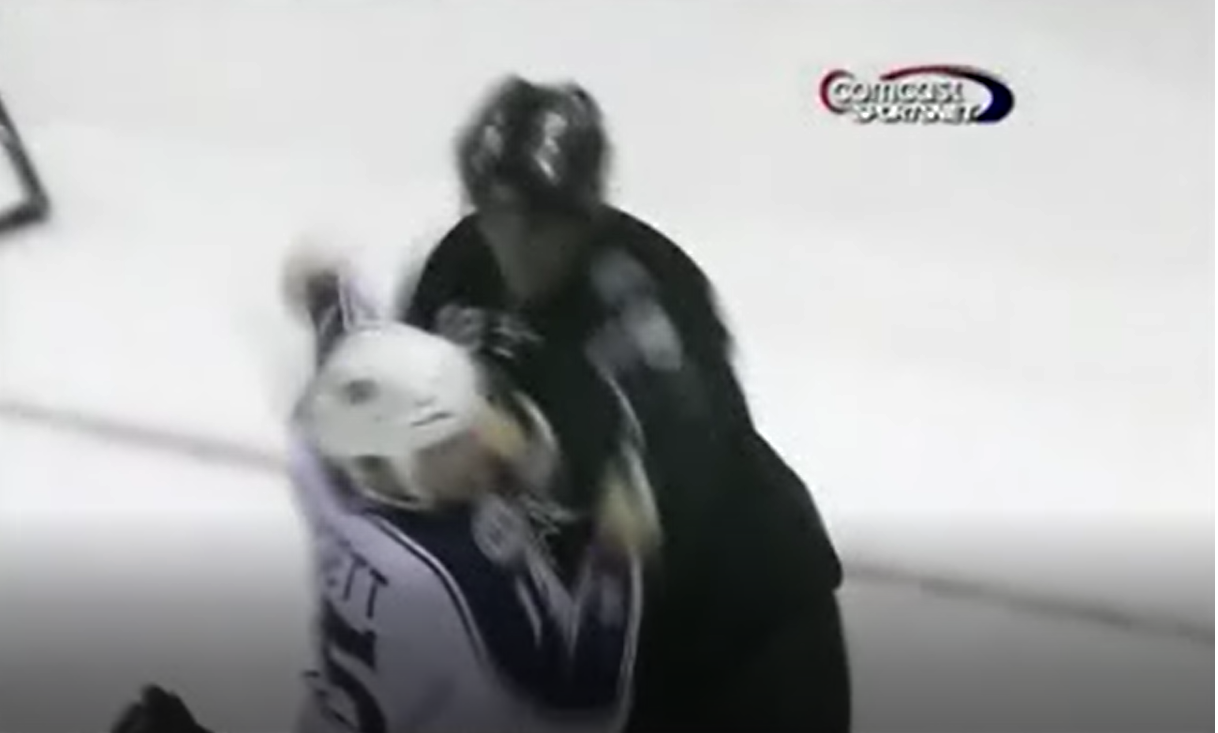
\includegraphics[width=6cm]{images/hockeyFight.png} }}%
    \qquad
    \subfloat[\centering Frame no conteniendo violencia]{{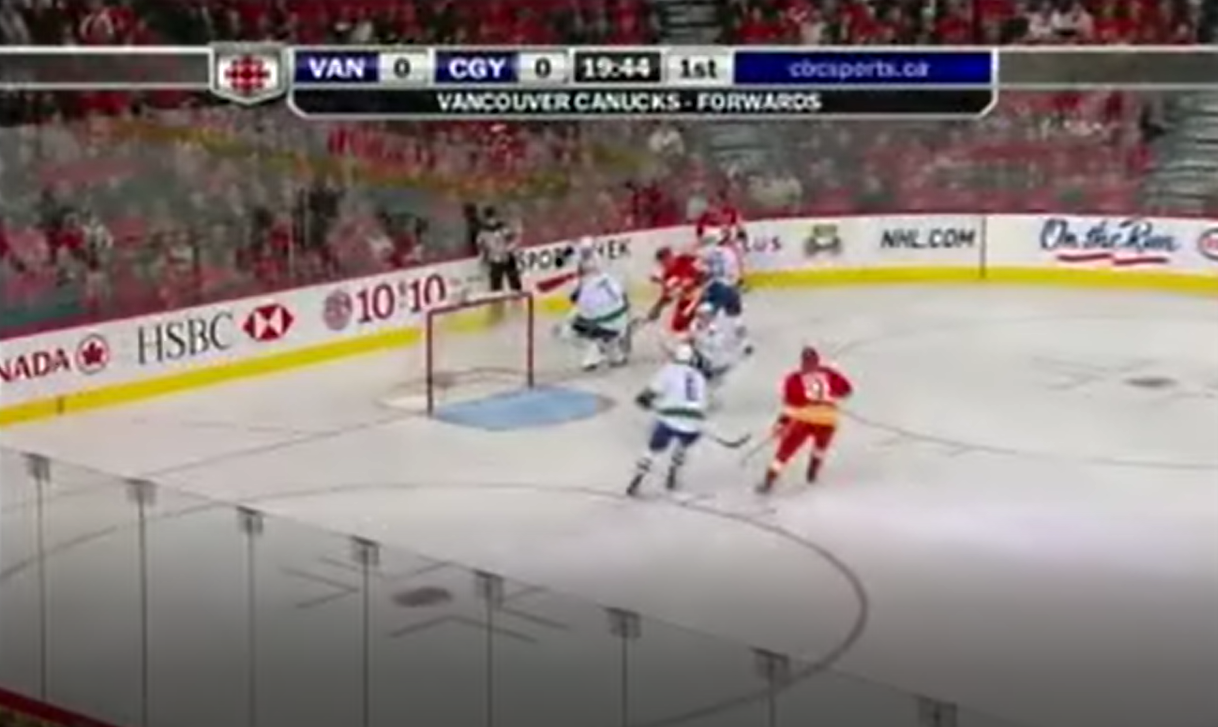
\includegraphics[width=6cm]{images/hockeyNotFight.png} }}%
    \caption{Comparación entre frames con y sin violencia en el ``\textit{Hockey Fight Detection Dataset}'' }%
    \label{fig:combinedHockey}%
\end{figure}

Este \textit{dataset} es escogido debido a que ya ha sido explorado 
a profundidad en el estado del arte, tal como fue explicado en 
el Capítulo \ref{contexto}, gracias a su facilidad de clasificación, 
estabilidad de los resultados (95\% o más) y la homogeneidad de las 
clases a clasificar. Estas cualidades nos permite tener una base 
estable para poder evaluar el efecto que tienen las capas Bi-LSTM y 
poder evaluar el cambio de las métricas con respecto a las difernetes 
experimentaciones a realizar.

\subsection{\textit{Pipeline} propuesto} \label{pipeline}

La Imagen \ref{metodologia} ilustra la metodología propuesta, 
la cual se procede a explicar a continuación:

\begin{figure}[h!] 
    \includegraphics[width=0.9\textwidth]{images/metodologiaMaestria.png} 
    \centering 
    \caption{Metodología propuesta.} 
    \label{metodologia} 
\end{figure}

En la Sección A se especifica el mecanismo de preprocesamiento 
que se utiliza para el trabajo, conteniendo un \textit{pipeline} con 
los siguientes pasos: recorte, redimensionamiento, normalización, 
etiquetado y filtrado.\\

En la Sección B se detalla la eleccion de la CNN a utilizar en el 
\textit{pipeline} mencionado en la seccion A y que permitirá 
extraer las características de los \textit{frames} de los videos 
a clasificar.\\

En la Sección C se mencionan las métricas con las que se evaluará el 
\textit{pipeline}, el proceso de entrenamiento y prueba y cuales 
serán las casuísticas con las cuales se experimentará con el 
\textit{pipeline}.\\

\textbf{A) Pre-procesamiento del \textit{dataset}}\label{procesamiento}\\

Como primer paso, se descarga el \textit{dataset} a 
través de su repositorio de 
\href{https://www.kaggle.com/datasets/yassershrief/hockey-fight-vidoes/data}{Kaggle}. 
El repositorio cuenta con una carpeta con todos los videos, 
los cuales incluyen archivos mp4 con los frames de cada uno 
de los videos. A continuación se lista cada uno de los pasos estructurados 
en varias etapas para preparar el \textit{dataset} y 
garantizar su compatibilidad con los modelos de aprendizaje 
profundo utilizado:

\begin{itemize}

    \item \textbf{Recorte y redimensionamiento}: Los frames 
    que se extraen se redimensionan a una resolución fija 
    (como 224x224 píxeles), adaptándose así a los 
    requerimientos de entrada de los modelos de red neuronal 
    convolucional (CNN) en la etapa de extracción 
    de características.

    \item \textbf{Normalización}: Con el objetivo de mejorar 
    la eficiencia del entrenamiento de los modelos, se 
    normalizan los valores de los píxeles de las imágenes. 
    Esto se realiza escalando los valores del rango [0, 255] 
    al rango [0, 1] o aplicar una normalización estadística 
    basada en la media y desviación estándar de los canales 
    RGB, especialmente útil cuando se emplean modelos 
    preentrenados.

    \item \textbf{Etiquetado de los datos}: A partir de los 
    nombres de los videos y su contexto, se asignan etiquetas 
    binarias a cada secuencia de imágenes. Esto es facilmente 
    reconocible debido a que aquellos videos que comiencen con 
    ``fi'' contienen violencia, mientra que los demás, no. 
    Los videos son  clasificados como \textit{violentos} o 
    \textit{no violentos}, y dicha etiqueta se propaga a 
    todos los frames correspondientes al video, asumiendo 
    homogeneidad del contenido en cada segmento.

    \item \textbf{Filtrado y muestreo}: El número total de frames por 
    video es variable, pero en el rango de 40-50 frames.
    Para reducir la redundancia y el volumen de datos, se aplica una 
    estrategia de muestreo temporal, extrayendo únicamente un 
    subconjunto de los frames. Para ello, se propone un 
    muestreo con reemplazo en donde se registra un número final 
    de frames y se procede a obtener un frame cada x de los videos. 
    Para el presente trabajo, se obtienen 10 frames (1 de cada 4-5 
    dependiendo del número original que contiene ese video) de manera 
    estandar para cada uno de ellos. Esto es util no solo para el 
    \textit{dataset} actual, sino para que sea utilizado en 
    otros ejemplares.
\end{itemize}

Este pre-procesamiento es esencial para estandarizar 
los datos, minimizar el ruido y facilitar el posterior 
entrenamiento de los modelos de detección de violencia basados 
en aprendizaje profundo.\\

\textbf{B) Extractor de características a través de CNN's}\label{extraccion}\\

A continuación se detalla la elección del extractor de características
basado en CNN's, las razones y las modificaciones necesarias para 
poder ser utilizadas con los datos preprocesados en la anterior Sección.\\ 

Para comenzar, se evalúan diferentes arquitecturas usadas en la 
actualidad. En 2020, Orhan Yalsin \cite{DataModelos} realizó un resumen 
con algunas métricas para la evaluación de diferentes 
modelos de vanguardia, los cuales son mostrados 
en la Tabla \ref{evaluacion}. Nos basamos en sus resultados 
para seleccionar aquellos modelos que son mas eficientes 
tanto en tiempo, espacio y precisión. Cabe resaltar que la 
tabla ha sido recortada para mencionar únicamente los modelos que nos interesan.\\

\begin{table}[h!]
\centering
\footnotesize
\begin{tabular}{|l|r|r|r|r|r|}
\hline
\textbf{\textit{Model}}                                         & \textbf{\textit{Size}}            & \textbf{\textit{Top-1 Accuracy}}                                                          & \textbf{\textit{Top-5 Accuracy}}                                                          & \textbf{\textit{Parameters}}           & \textbf{\textit{Depth}}          \\ \hline
    Xception                                                     & 88 MB                              & 0.790                                                                                   & 0.945                                                                                   & 22,910,480                               & 126                                 \\ \hline
    VGG19                                                        & 549 MB                             & 0.713                                                                                   & 0.900                                                                                   & 143,667,240                              & 26                                  \\ \hline
    ResNet50                                                     & 98 MB                              & 0.749                                                                                   & 0.921                                                                                   & 25,636,712                               & -                                   \\ \hline
    InceptionV3                                                  & 92 MB                              & 0.779                                                                                   & 0.937                                                                                   & 23,851,784                               & 159                                 \\ \hline
    MobileNet                                                    & 16 MB                              & 0.704                                                                                   & 0.895                                                                                   & 4,253,864                                & 88                                  \\ \hline
    MobileNetV2                                                  & 14 MB                              & 0.713                                                                                   & 0.901                                                                                   & 3,538,984                                & 88                                  \\ \hline
    EfficientNetB0                                               & 29 MB                              & 0.771                                                                                   & 0.933                                                                                   & 5,330,571                                & -                                   \\ \hline
    EfficientNetB1                                               & 31 MB                              & 0.791                                                                                   & 0.944                                                                                   & 7,856,239                                & -                                   \\ \hline
    EfficientNetB2                                               & 36 MB                              & 0.801                                                                                   & 0.949                                                                                   & 9,177,569                                & -                                   \\ \hline
    EfficientNetB3                                               & 48 MB                              & 0.816                                                                                   & 0.957                                                                                   & 12,320,535                               & -                                   \\ \hline
    EfficientNetB4                                               & 75 MB                              & 0.829                                                                                   & 0.964                                                                                   & 19,466,823                               & -                                   \\ \hline
    EfficientNetB5                                               & 118 MB                             & 0.836                                                                                   & 0.967                                                                                   & 30,562,527                               & -                                   \\ \hline
    EfficientNetB6                                               & 166 MB                             & 0.840                                                                                   & 0.968                                                                                   & 43,265,143                               & -                                   \\ \hline
    EfficientNetB7                                               & 256 MB                             & 0.843                                                                                   & 0.970                                                                                   & 66,658,687                               & -                                   \\ \hline
    \end{tabular}
    \caption[Evaluación de diferentes modelos. Tabla brindada por Orhan Yalcin.]
    {Evaluación de diferentes modelos. Tabla brindada por Orhan Yalcin \protect\cite{DataModelos}.}
    \label{evaluacion}
\end{table}

La Tabla \ref{evaluacion} destaca varios modelos notables por su equilibrio entre 
tamaño, cantidad de parámetros y precisión. Entre ellos VGG19 
(si consideramos solo las capas convolucionales), ResNet50, InceptionV3, 
y los EfficientNetBX resultan tener una buena relación entre el peso, el 
número de parámetros y la precisión que estas obtienen, esta última 
siendo de las más altas dentro de todos estos modelos. Se tuvo en 
consideración la ejecución en videos en tiempo real y por ello es necesario 
que el modelo sea el más pequeño posible evitando perder la precisión. También 
por ello, están las MobileNet, las cuales ya han sido utilizadas para el 
procesamiento de imágenes en tiempo real por ser más ligeras, enfocadas a 
ser utilizadas en celulares. Todas estas redes eran aptas para 
este problema y pasarán a ser evaluadas en el siguiente capítulo, en base 
al primer \textit{dataset} mencionado anteriormente. \\

Para reforzar esta elección, se utiliza el resultado obtenido en un trabajo previo 
de mi autoría, titulado ``\textit{Machine Learning Pipeline} Para el 
Etiquetado Automático en Imágenes de Especies de Peces Peruanos''
\cite{Madera2024}, en donde se experimentó con todas las 
redes anteriormente mencionadas para la tarea de clasificación de imágenes 
de peces peruanos. La Tabla \ref{table:data1} referencia los resultados 
obtenidos en aquella experimentación:

\begin{table}[h!]
    \footnotesize
    \centering
    \begin{tabular}{|c|c|c|c|c|c|c|}
    \hline
    \textbf{} & \textbf{\begin{tabular}[c]{@{}c@{}}Precisión\\en\\training\end{tabular}} & \textbf{\begin{tabular}[c]{@{}c@{}}Precisión \\ en \\ validation\end{tabular}} & \textbf{\begin{tabular}[c]{@{}c@{}}Precisión \\ en \\testing\end{tabular}} & \textbf{\begin{tabular}[c]{@{}c@{}}Perdida \\ final en \\ training\end{tabular}} & \textbf{\begin{tabular}[c]{@{}c@{}}Velocidad \\ por batch\\ (8 \\imágenes) \\ en ms\end{tabular}} & \textbf{\begin{tabular}[c]{@{}c@{}}Número \\ de\\ épocas\end{tabular}} \\ \hline
    \textbf{Vgg19} & 0.9193 & 0.9928 & 0.9926 & 0.2299 & 71 & 21 \\ \hline
    \textbf{Resnet50} & \textbf{0.9596} & \textbf{0.9993} & 0.9950 & 0.1282 & 52 & 14 \\ \hline
    \textbf{\begin{tabular}[c]{@{}c@{}}Inception\\V3\end{tabular}} & 0.7362 & 0.6620 & 0.6681 & 0.6901 & 42 & 40 \\ \hline
    \textbf{\begin{tabular}[c]{@{}c@{}}MobileNet\\V2\end{tabular}} & 0.8521 & 0.9052 & 0.9104 & 0.4143 & 28 & 31 \\ \hline
    \textbf{\begin{tabular}[c]{@{}c@{}}MobileNet\\V1\end{tabular}} & 0.8694 & 0.9288 & 0.9519 & 0.3628 & \textbf{23} & 23 \\ \hline
    \textbf{Xception} & 0.7244 & 0.7085 & 0.7178 & 0.7490 & 48 & 25 \\ \hline
    \textbf{\begin{tabular}[c]{@{}c@{}}EfficientNet\\B0\end{tabular}} & 0.9577 & \textbf{0.9993} & \textbf{1.0000} & \textbf{0.1270} & 41 & \textbf{19} \\ \hline
    \end{tabular}
    \caption{Datos obtenidos de la experimentación previa con \textit{dataset} de peces }
    \label{table:data1}
\end{table}

En la Tabla \ref{table:data1} se puede ver como los mejores resultados 
fueron obtenidos por EfficientNetB0 y Resnet50 tanto en precisión, velocidad 
por batch y épocas de entrenamiento, por lo que se usan para 
el presente trabajo. Para darle más variablidad al presente trabajo, se 
escoge MobilenetV3 como modelo control y además, EfficientnetV2, el 
cual es un modelo un poco más pesado pero que brinda una 
gran mejora en la precisión general a comparación de 
EfficientNetB0. Cabe resaltar que para cada una de estas redes 
se aplica un proceso de \textit{transfer-learning}, por lo que 
no es necesario entrenar ni probar con los datos, sino que solo va a 
ser utilizado para obtener el vector característico de cada uno de 
los frames. Para poder entender mejor la estructura de cada una de 
estas redes, a continuación se detallan cada una de ellas. \\

\textbf{\underline{ResNet50}} \\

Creado por Microsoft en 2015, este modelo también cuenta con 50 capas de
profundidad. Emplea una técnica llamada \textit{residual learning}
\cite{He2015}, que consiste en guardar una copia de la salida actual y
sumarla al resultado obtenido de un conjunto de convoluciones (típicamente
cada tres). La Figura \ref{ResNet} ilustra esta modificación y la arquitectura
general del modelo. Este modelo también fue probado en el mismo
\textit{dataset}, obteniendo una precisión del 92.1\%, y el aprendizaje
residual evitó un aumento en la dimensionalidad del modelo.
Contiene aproximadamente 25.6 millones de parámetros y ocupa 98 MB de 
memoria.

\begin{figure}[h!] 
    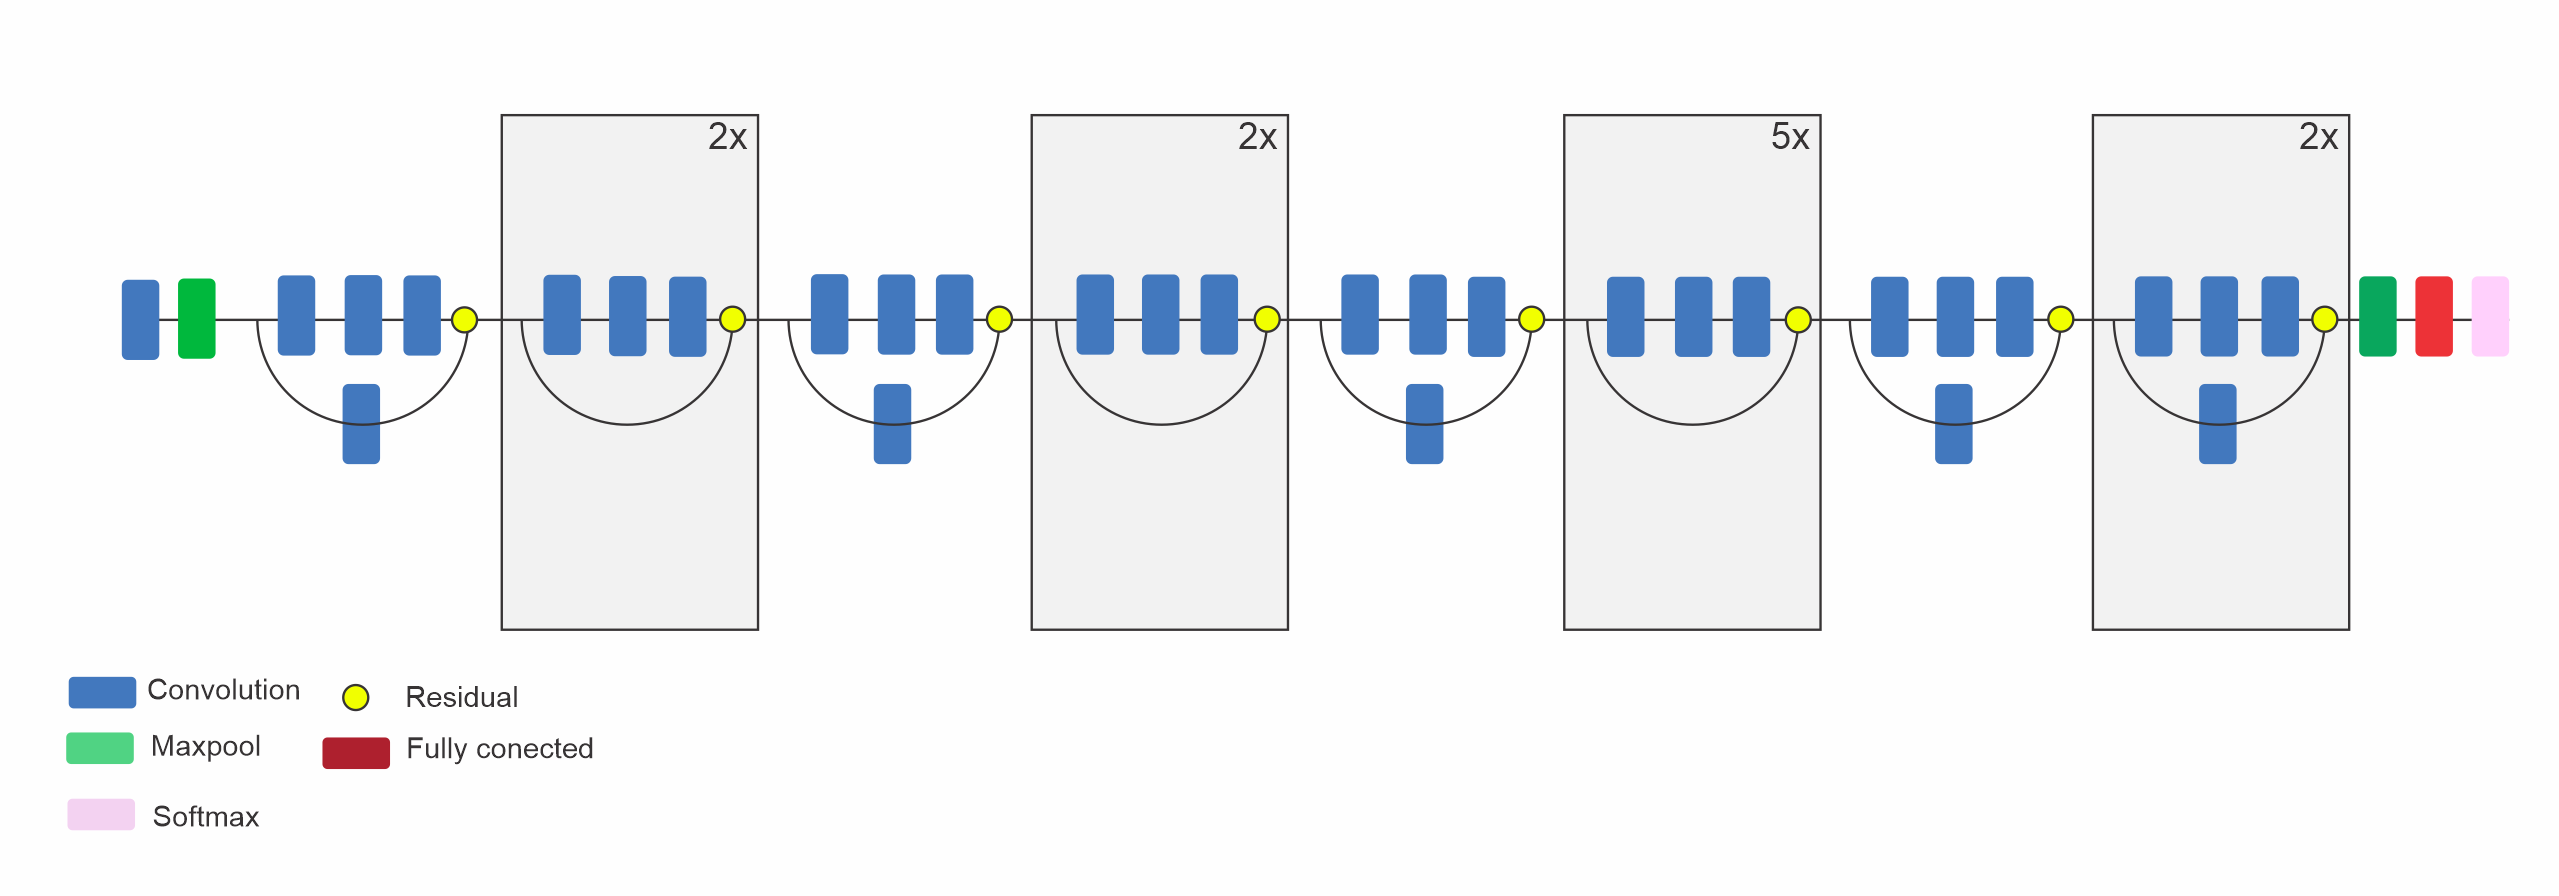
\includegraphics[width=1\textwidth]{images/ResNet.png} 
    \centering 
    \caption[Versión simplificada de ResNet50]
    {Versión simplificada de ResNet50 \protect \cite{modelos}.}
    \label{ResNet} 
\end{figure}

\textbf{\underline{MobileNetV3Large}} \\

MobileNetV3 fue creado en el paper \textit{Searching for MobileNetV3} 
\cite{Howard2019}. Es una arquitectura propuesta en 2019 enfocada en 
dispositivos con recursos limitados. Esta versión representa la tercera 
iteración de la familia MobileNet, que es diseñada para mantener un 
equilibrio entre precisión y eficiencia computacional, optimizando el 
rendimiento en dispositivos móviles o embebidos.\\

Esta arquitectura presenta dos variantes principales: MobileNetV3-Small 
y MobileNetV3-Large. MobileNetV3-Small está orientada a tareas con bajo 
consumo de recursos, con aproximadamente 2.5 millones de parámetros y 
una precisión cercana al 67.4\% en ImageNet. En contraste, MobileNetV3-Large, 
con cerca de 5.4 millones de parámetros, logra una precisión del 75.2\% en 
el mismo conjunto de datos.\\

Esta arquitectura introduce mejoras clave como:
\begin{itemize}
    \item El uso de bloques \textit{Mobile Inverted Bottleneck} con 
    capas \textit{depthwise separable convolutions}.
    \item La incorporación de la función de activación \textit{Hard-Swish}, 
    más eficiente que la ReLU6 utilizada anteriormente.
    \item La integración del módulo de atención 
    \textit{SE block (Squeeze-and-Excitation)} para mejorar la 
    representación de características.
\end{itemize}

MobileNetV3 fue desarrollada mediante una combinación de algoritmos 
de búsqueda automática de arquitectura (NAS) y principios heurísticos, 
permitiendo encontrar configuraciones óptimas en términos de precisión 
y eficiencia. \\

La Figura \ref{MobileNetV3} ilustra la arquitectura general de MobileNetV3-Large.

\begin{figure}[h!] 
    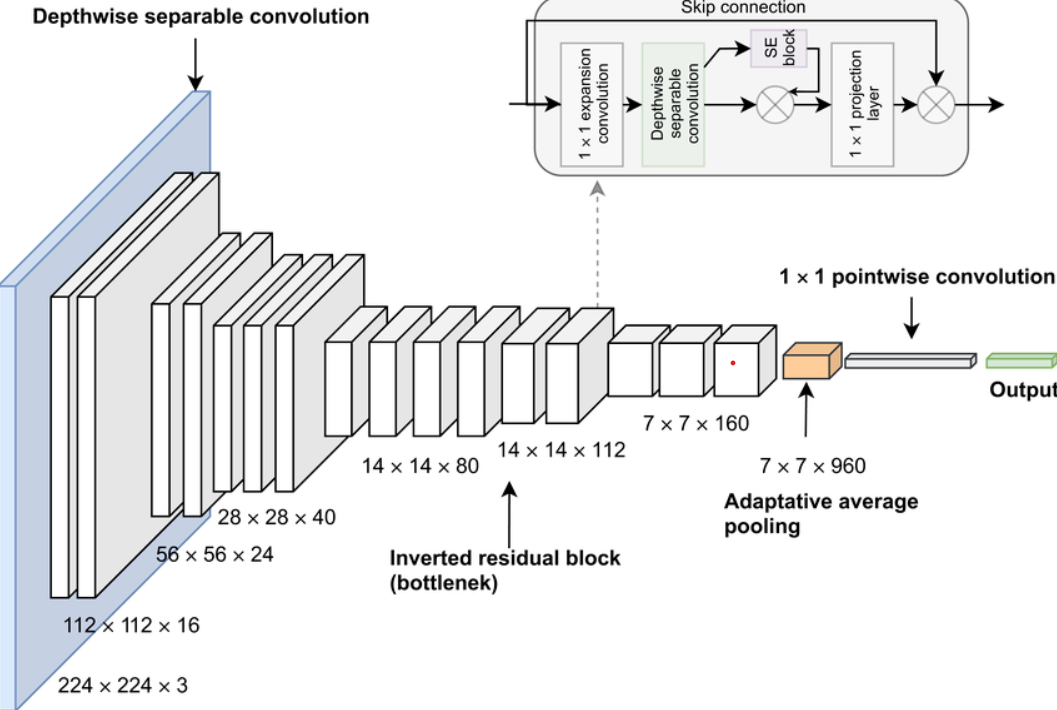
\includegraphics[width=0.5\textwidth]{images/MobileNetV3.png} 
    \centering  
    \caption[Versión simplificada de MobileNetV3.]
    {Versión simplificada de MobileNetV3 \protect \cite{AbdElaziz2024}.}
    \label{MobileNetV3} 
\end{figure}

\textbf{\underline{EfficientNet}} \\

EfficientNet es un conjunto de arquitecturas diseñadas por 
google en el paper ``\textit{EfficientNet: Rethinking Model Scaling for 
Convolutional Neural Networks}'' \cite{Tan2020} en 2020, 
consiste en 8 implementaciones diferentes (B0 a B7).
La versión más ligera (B0) contiene aproximadamente 5.5 
millones de parámetros y logró un 93\% de precisión en el 
mismo \textit{dataset}. Otras versiones continúan aumentando 
el número de parámetros y la precisión resultante. Comparado 
con los modelos anteriores, EfficientNetB4 con 19.5 millones 
de parámetros alcanza un 96.4\% de precisión, superándolos.
Este modelo optimiza su aprendizaje mediante un algoritmo de 
aproximación que genera parámetros para crear cada uno de 
los ocho modelos. Este algoritmo considera tres factores:
\begin{itemize} 
    \item Profundidad de las capas 
    \item Ancho de las capas (capas múltiples) 
    \item Resolución de la imagen 
\end{itemize} 

La Figura \ref{EfficientNetB0} muestra la estructura de 
EfficientNetB0.\\

\begin{figure}[h!] 
    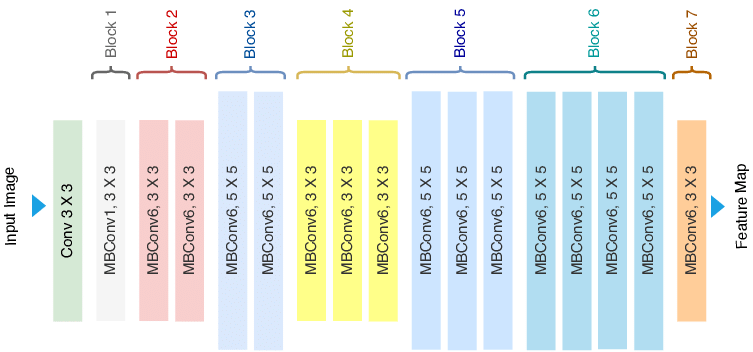
\includegraphics[width=1\textwidth]{images/EfficientNetB0.png} 
    \centering 
    \caption[Versión simplificada de EfficientNetB0.]
    {Versión simplificada de EfficientNetB0 \protect \cite{EfficientNetB0}.}
    \label{EfficientNetB0} 
\end{figure}

\textbf{\underline{EfficientNetV2}} \\

EfficientNetV2 fue creado en el paper \textit{EfficientNetV2: Smaller Models 
and Faster Training} \cite{Tan2021} es una evolución de la arquitectura 
EfficientNet propuesta en 2021. Esta versión mejora tanto la eficiencia 
como la velocidad de entrenamiento mediante el uso de técnicas avanzadas 
de regularización y una arquitectura optimizada.\\

EfficientNetV2 introduce tres variantes principales: S (Small), M (Medium) 
y L (Large), diseñadas para ajustarse a distintos compromisos entre precisión 
y costo computacional. Por ejemplo, EfficientNetV2-S contiene alrededor 
de 24 millones de parámetros y alcanza una precisión del 83.9\% en ImageNet, 
mientras que EfficientNetV2-L, con aproximadamente 120 millones de parámetros, 
logra una precisión del 85.7\%.\\

Una de las mejoras clave en esta versión es el uso del bloque \textit{Fused-MBConv}, 
que combina convoluciones estándar y convoluciones móviles en las primeras 
capas, lo cual reduce el tiempo de entrenamiento. Además, se utiliza un 
enfoque de escalado progresivo para entrenar los modelos más eficientemente. 
Además cuenta con las mismas optimizaciones que la versiones EfficientNetBX.\\

La Figura \ref{EfficientNetV2} muestra la arquitectura general de EfficientNetV2-S. \\

\begin{figure}[h!] 
    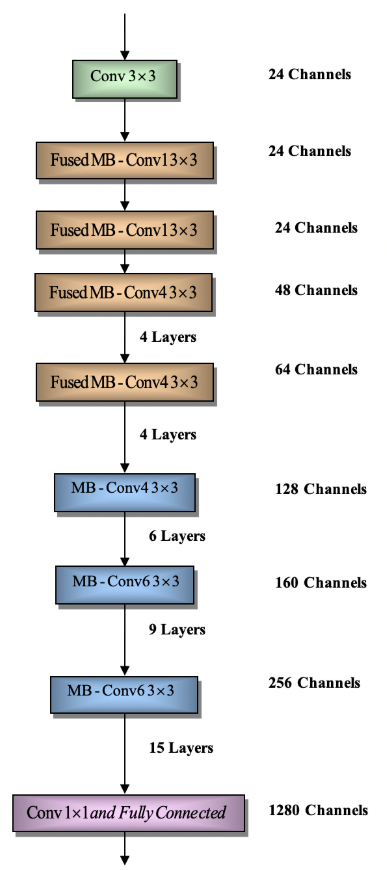
\includegraphics[width=0.5\textwidth]{images/EfficientNetV2.png} 
    \centering 
    \caption[Versión simplificada de EfficientNetV2.]
    {Versión simplificada de EfficientNetV2 \protect \cite{AlTakrouri2023}.}
    \label{EfficientNetV2} 
\end{figure}

\textbf{C) Entrenamiento y prueba del clasificador}\label{entrenamiento}\\

Como clasificador, se utilizan modelos BI-LSTM con diferente 
número de celdas. Para esta experimentación, se decidió usar 
un número entre 1 y 9 celdas, ya que consistía en un dataset 
bastante sencillo utilizado y estudiado en el estado del arte 
anteriormente mencionado. En los artículos revisados en el 
Capítulo \ref{contexto}, se utilizan un número 
relativamente bajo de capas Bi-LSTM (10-40) con modelos de 
CNN no actualizados. Es por ello que se planea utilizar un 
número de capas menor para evitar tener un problema de 
overfitting. Además, reducir el número de capas Bi-LSTM 
ayuda en la reducción del tiempo de inferencia, lo cual es 
esencialmente bueno para el contexto en el que se está usando 
este tipo de \textit{pipelines}.\\

Para cada uno de las CNN's que se mencionan en la anterior Sección, 
y para cada una de las configuraciones de celdas, se procedió a 
entrenar y testear cada combinación de ellas. Las consideraciones 
para este modelo son las siguientes:

\begin{itemize}
    \item De entrada se tienen los vectores de características 
    obtenidos del paso anterior (se debe considerar que los 
    tamaños de salida puden variar con respecto a la CNN). 
    \item Se crea un modelo BI-LSTM con X celdas, 10 timesteps 
    (10 frames extraídos del preprocesamiento) y el tamaño 
    del output del anterior paso.
    \item Capas densas de 1024, 50 y 2 neuronas con funciones 
    de activación RelU y la última de tipo softmax. 
    \item Función de pérdida Binary CrossEntropy, optimizador adam 
    y de métricas \textit{accuracy} y \textit{f1-score}.
    \item Función de early stopping con \textit{patience} de 3 y  
    \textit{min delta} de 0.005 y batch de 16 videos por vez.
\end{itemize}

En la siguiente sección se presentarán los resultados 
generados utilizando las anteriores consideraciones para 
cada uno de los modelos mencionados.

\subsection{Métricas de Evaluación}

Para la evaluación del conjunto de datos 
\textit{Jockey Fights}, se utilizan las siguientes 
métricas de rendimiento:

\begin{itemize}
    \item \textbf{Accuracy}: mide la proporción de predicciones 
    correctas respecto al total de predicciones realizadas. Es 
    una métrica general útil cuando las clases están balanceadas 
    como en el nuestro.
    \begin{equation}
        \text{Accuracy} = \frac{\text{True Positives} + \text{True Negatives}}{\text{Total Predictions}}
    \end{equation}
    \item \textbf{Tiempo de Inferencia}: Mide el tiempo que 
    el modelo tarda en procesar una secuencia completa o un 
    solo frame. Es crucial para aplicaciones en tiempo real 
    o streaming.

\end{itemize}
